\chapter{INTRODUCTION}




\section{Communication matters}

We live in a world where we are almost always connected to internet. Most of the people are using a smartphone. They can connect their phones to a cellular network owned by an operator such as Vodafone, Telstra or Optus in Australia and go to internet, send text or call a close relation. We now live in a world where we can communicate with anyone on the planet at almost anytime.\\
Communication has become a need for us. Daily we are communicating with people far from us. It can be for our job. We might be working in a team spread across multiple cities or country. It can be with our family and friends. Whatever the case, communication is crucial. We want to be able to contact someone at anytime and anywhere.\\
There is one situation where communication matters the most: during disasters whether they are natural (earthquakes, storm, tsunami, …) or not (terrorist attack). During such events, emergency services need to be able to communicate. Indeed, to save people’s lives, they must work very efficiently. Thus, they need to communicate so they can organise their team work.\\
For all these reasons, we should be able to communicate at anytime and anywhere.





%%%%%%%%%%%%%%%%%%%%%%%%%%%%%%%%%%%%%%%%%%%%%%%%%%%
%								Next Section 											%
%%%%%%%%%%%%%%%%%%%%%%%%%%%%%%%%%%%%%%%%%%%%%%%%%%%

\section{Reality is different}

We would like to be able to call our family at anytime and everywhere in the world. However, it’s still not possible. To be able to call someone you currently need some sort of connection to a cellular network. But these networks don’t cover the whole land even in a country as developed as Australia. One of the three big Australian operator, Telstra, display a map showing their current coverage on their website

\begin{figure}[H]
	\centering
	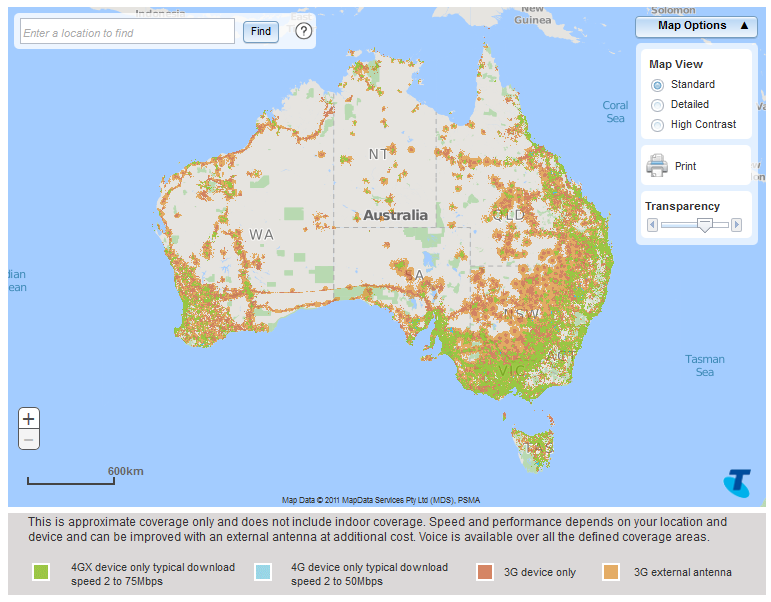
\includegraphics[width=0.6\textwidth]{image/Teslra-coverage.png}
	\caption{Telstra cellular coverage (Telstra.com.au, 2018)}
	\label{fig:Telstra}
\end{figure}

As we can see on the previous figure, Telstra cellular network is far from covering all Australia. Telstra network only covers places where people live. Telstra has no interest in places where no one live. Indeed, why would they extend their network in a part of Australia where no one live. They will just lose money: investment with no new customers at the end. 
Before extending its coverage, an operator mainly looks at two points: how much money will it cost and how many new customers will I get. If after studying these two points, they realise that they will never get back the money they invested, then they won’t spread their coverage. This means that small isolated towns may never have any connection with the rest of the world.
Right now, you cannot communicate anywhere. Unfortunately, even the covered zone cannot communicate all the time.
Indeed, in several cases, the network will go down. The few main reasons for a network to go down are the following:
\begin{itemize}
	\item Natural disasters (earthquake, storm, tsunami, ….).
	\item Human disasters (terrorist attacks).
	\item Network congestion
\end{itemize}
	
Looking at the past news, it is easy to find natural disasters where a huge part of the network went down. For instance, in august 2017, the tropical storm Harvey destroyed a huge part of the mobile network in Texas (Brodkin, 2017). First, this hurricane “has caused outages for more than 148,000 Internet, TV, and phone customers” leaving this people unable to make call. But, more importantly, this storm has damaged more than “17 emergency call centers”. During a hurricane, being able to call emergency centre can be a matter of life and death. When 17 call centres are disturbed by a storm, it means rescue teams might not be as effective as they can be. 

A good example of human disaster which had a tremendous impact for the emergency services is the bombing in London in 2005 (London.gov.uk, 2007). During this event, the carrier networks went down. Indeed, because of the bombs, a lot of people used their phones to call their families and close relations. This led to a network congestion. The network had reached his full capacity and couldn’t be used by the emergency staff. 

As we can see from the few examples above, we still cannot communicate at anytime and anywhere. These examples also demonstrate the importance of communication. In addition to be a need for us, it can also save lives. Therefore, we should try to find a way to provide a system of communication which is available all the time and everywhere.
This kind of communication services is the purpose of an existing project: the Serval project. 





%%%%%%%%%%%%%%%%%%%%%%%%%%%%%%%%%%%%%%%%%%%%%%%%%%%
%								Next Section 											%
%%%%%%%%%%%%%%%%%%%%%%%%%%%%%%%%%%%%%%%%%%%%%%%%%%%

\section{Presentation of the Serval Project}
\subsection{Purpose of the project}

The Serval Project started 8 years ago. What inspired Paul Gardner-Stephen and Romana Challans to launch this project is the Haiti earthquake that happened in 2010 (Encyclopedia Britannica, 2017) (Gardner-Stephen et al., 2013). During this event, most of the cellular networks went down. Without any communication means, the rescue team had a lot of trouble to organise which led to more casualties. Therefore, the goal of the Serval Project is to offer a way of communication when the common ones are dysfunctional or unavailable.

In other words, they want to create a communication system available everywhere and at anytime.

To reach that goal, the solution must be low-cost. Indeed, if one wants to install a system everywhere it should be easy and cheap to deploy.



%%%%%%%%%%%%%%%%%%%%%%%%% Next Subsection

\subsection{Structure of the project}

The Serval Project uses the following structure:

\begin{figure}[H]
	\centering
	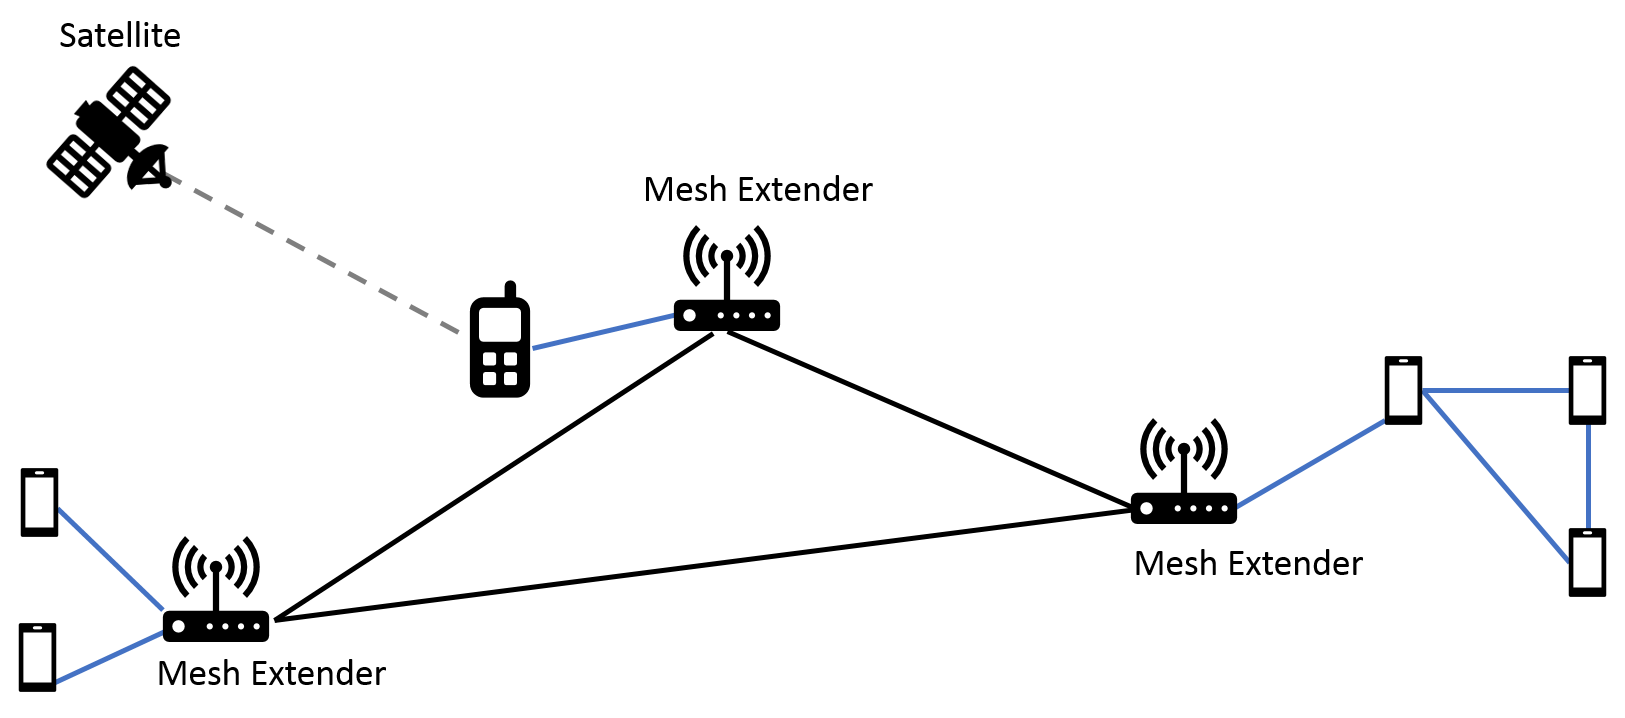
\includegraphics[width=0.6\textwidth]{image/Infra.png}
	\caption{Serval project structure}
	\label{fig:struct}
\end{figure}

\begin{tabular}{r@{: }l r@{: }l}
Legend & \\
\tikz[baseline]{\draw[ultra thick] (0,.5ex)--++(.5,0) ;}& UHF \\
\tikz[baseline]{\draw[ultra thick, color=blue] (0,.5ex)--++(.5,0) ;}& Wi-Fi\\
\tikz[baseline]{\draw[ultra thick, dashed] (0,.5ex)--++(.5,0) ;}& Satellite communication
\end{tabular}

As we can see on the previous picture, the Serval project uses a mesh network. A mesh network is a network where all the nodes are dynamically making connections with as many other nodes as possible. In the Serval project, the nodes are typically mobile phones, mesh extenders or devices for satellite connection.

This kind of structure has a few advantages. The connections are dynamically constructed which means that the network is easily scalable. Furthermore, since each device try to create as many links as possible, there are a lot of redundancy in the network. So even if a path between two devices breaks, there are still plenty other paths for the two phones to communicate.
The smartphones are using Wi-Fi to communicate which means that any person with a cellular can join the network by using an open-source, free application. 

However, Wi-Fi has a small range. In perfect conditions (free-space), Wi-Fi can reach around 200m. But in reality, in the best-case scenario, we can expect 80 to 100 m outdoor and 20 to 30m indoor. If the Wi-Fi was only used to interconnect the mobiles, the network wouldn’t reach very far. Thus, the mesh extenders were added. 
As their name suggest, the goal of the mesh extender is to extend the reach of the network. They are composed of 2 antennas:
\begin{itemize}
		\item A Wi-Fi antenna used for the communication between the user’s devices and the mesh extender
		\item A radio antenna, used between the mesh extenders
\end{itemize}


The radio transmission is designed to have a very long range (greater than 3km (Gardner-Stephen et al., 2013)). The mesh extenders play an important role in the project. They allow two users, who are very far from one and another, to communicate. Since they should be deployed at many places, they are designed to be low-cost and self-sufficient (for instance, solar panel can be used to power them). 

The last component of the structure is the satellite communication. This part is still not finished and is one of the upcoming project.

This structure allows the users to communicate by using an application (Serval Mesh).



%%%%%%%%%%%%%%%%%%%%%%%%%%%%%%%%%%%%%%%%%%%%%%%%%%%
%								Next Section 											%
%%%%%%%%%%%%%%%%%%%%%%%%%%%%%%%%%%%%%%%%%%%%%%%%%%%

\section{Statement of the problem}

Even though a lot of work has been done since 2010, the project is still not over yet. Therefore, there are still some faults, failures. 
Last year, there was a pilot deployment in Vanuatu. This pilot revealed some software and hardware faults and failures within the mesh extenders. These faults mean that in some cases, the mesh network doesn’t work and no communication is available. Therefore, the goal of the project (offering a system of communication when the usual ones fail) is not reached yet. 
In order to fix the found faults, you need to be able to recreate them. Currently, the team, here at Tonsley, lacks a real environment testbed to reproduce these faults and find new ones. Therefore, the goal of my project is to design a complete, practical test network for the Mesh Extenders and deploy it in Tonsley.

Through my project I will try to answer the following research questions:
\begin{itemize}
	\item How to design a test network for a Mesh Extender?
	\item What are the key points such testbed should answer?
	\item How can we be sure the testbed is not affecting the Mesh Extender normal functioning?
\end{itemize}
